\documentclass{article}
\usepackage{graphicx}

\setlength{\parindent}{0pt}

\begin{document}

\title{UADE 2.xx design specification}
\author{Heikki Orsila $<$heikki.orsila@iki.fi$>$}
\date{}
\maketitle

\section{Introduction}

\subsection{History}

UADE 1.xx was written to be a stand-alone program that had separate code
for each possible \emph{frontend} (\emph{user interface}), but there was
no internal structure to implement different frontends easily. By much
hacking some kind of pseudo-interface was created to facilitate following
frontends:
\begin{itemize}
  \item Beep Media Player
  \item MorphOS shell without interaction
  \item Unix shell without interaction
  \item Unix shell with small interaction
  \item XMMS plugin
\end{itemize}

It was a clear design problem that needed to be fixed. To force the separation
of frontend and emulator UADE 2.xx removed all user interface issues from
the emulator. Token-passing based messaging system was implemented into
the emulator. The frontend would communicate with the emulator through a
token-passing based messaging protocol that has following commands:
\begin{itemize}
\item foo
\end{itemize}


\begin{figure}
\centering
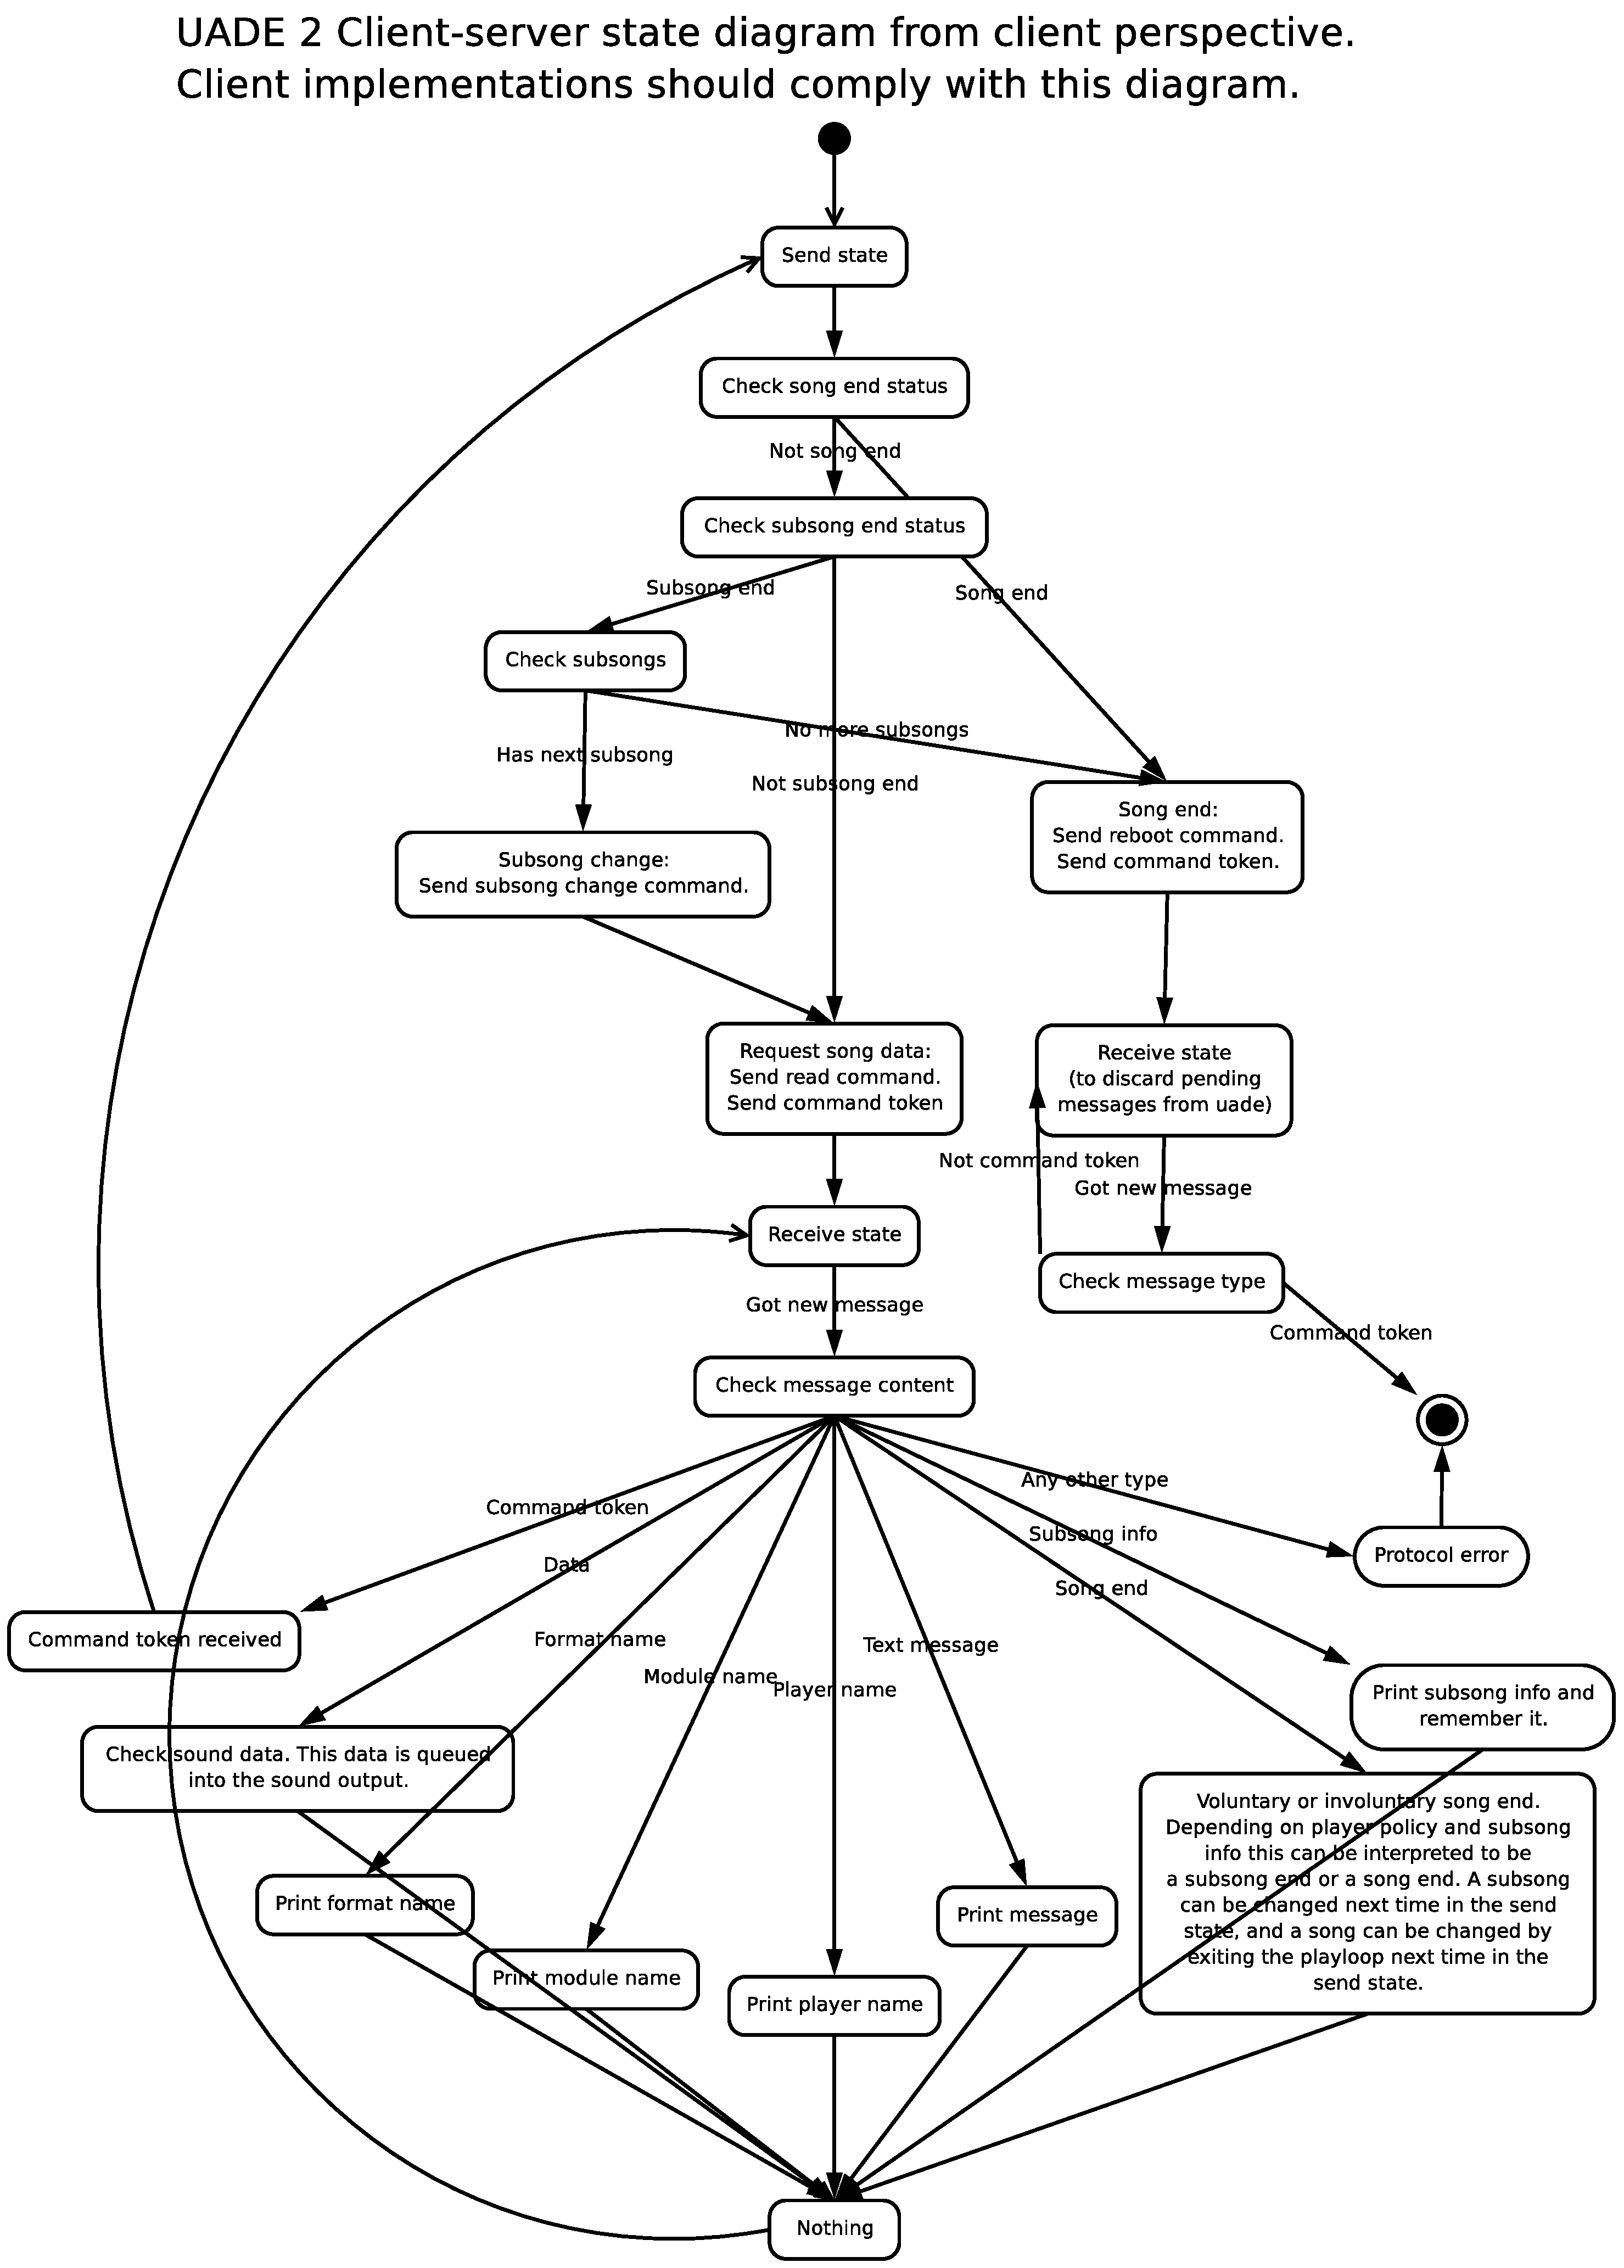
\includegraphics[scale=0.25]{play_loop_state_diagram.eps}
\caption{Play loop interaction from client (frontend) perspective}
\label{fig:playloop}
\end{figure}

\end{document}
